\section{Feature-Space Frame-0 Attack}
\label{sec:feature_exps}

Based on the Round 4 conclusion and UAP-SAM2~\citep{uap_sam2_2025}, which achieves $-45.8$ pp mIoU with feature-space objectives but does not test under H.264, we designed three feature-space attack modes targeting progressively deeper insertion points in SAM2's video pipeline.

\subsection{Experimental Setup}

All three modes use per-video Adam optimization of $\delta_0$ (300 steps, 2 restarts), with the official \texttt{SAM2VideoPredictor} for evaluation. We attack only frame 0; all later frames use the clean (original) video, compressed with H.264 CRF23. This is the most favorable setting for the attacker: if poisoning the single initial memory write cannot survive codec, a multi-frame attack also cannot.

\subsection{Results}

\cref{tab:per_video} shows per-video results for all three modes. \cref{fig:main_results} summarizes all experiments.

\begin{table}[t]
\centering
\small
\caption{Per-video results for all three feature-space attack modes on 9 DAVIS validation videos (CRF 23). $\Delta\text{JF}_\text{adv}$: tracking degradation without codec (↑ better attack). $\Delta\text{JF}_\text{auc}$: tracking degradation under CRF23 (↑ better attack). All $\Delta\text{JF}_\text{auc}$ values are near zero, confirming the codec-kill hypothesis.}
\label{tab:per_video}
\begin{tabular}{lc|cc|cc|cc}
\toprule
& & \multicolumn{2}{c|}{F0-B (FPN)} & \multicolumn{2}{c|}{F0-CD$_\text{nm}$} & \multicolumn{2}{c}{F0-CD (Full)} \\
Video & JF$_\text{clean}$ & $\Delta$JF$_\text{adv}$ & $\Delta$JF$_\text{auc}$ & $\Delta$JF$_\text{adv}$ & $\Delta$JF$_\text{auc}$ & $\Delta$JF$_\text{adv}$ & $\Delta$JF$_\text{auc}$ \\
\midrule
cows & 0.975 & -0.000 & -0.011 & +0.005 & -0.000 & +0.036 & +0.001 \\
car-turn & 0.954 & -0.004 & -0.001 & +0.002 & +0.004 & -0.011 & -0.000 \\
car-roundabout & 0.952 & +0.001 & -0.003 & -0.007 & -0.003 & -0.005 & -0.004 \\
crossing & 0.949 & -0.004 & -0.006 & -0.003 & -0.004 & -0.001 & -0.006 \\
bus$^\dagger$ & 0.935 & +0.019 & +0.014 & +0.016 & +0.015 & +0.867 & -0.002 \\
blackswan & 0.920 & +0.234 & -0.028 & -0.014 & -0.017 & -0.012 & -0.012 \\
classic-car & 0.804 & +0.103 & +0.020 & -0.055 & -0.056 & -0.056 & -0.018 \\
color-run & 0.800 & +0.481 & +0.029 & +0.371 & +0.023 & +0.005 & -0.005 \\
bike-packing & 0.739 & +0.260 & -0.047 & +0.029 & +0.018 & +0.033 & +0.006 \\
\midrule
\textbf{Mean} & 0.892 & +0.121 & -0.004 & +0.038 & -0.002 & +0.095 & -0.004 \\
\bottomrule
\end{tabular}
\begin{flushleft}
\footnotesize $\dagger$ Bus video: F0-CD achieves $\Delta$JF$_\text{adv}=+0.867$ (SAM2 tracking collapses from 93.5\% to 6.8\%), but $\Delta$JF$_\text{auc}=-0.002$ after CRF23.
\end{flushleft}
\end{table}

\paragraph{Mode F0-B (FPN feature shift).}
Mean $\djfadv = +0.121$ (some attack success without codec), mean $\djfauc = -0.004$ (CRF23). The FPN features shift substantially under the adversarial perturbation in the codec-free setting, but this shift is erased by H.264.

\paragraph{Mode F0-CD\textsubscript{nm} (maskmem + object pointer, no matching).}
Mean $\djfadv = +0.038$, mean $\djfauc = -0.002$ (CRF23). Targeting the actual written memory tokens rather than FPN output does not improve codec robustness.

\paragraph{Mode F0-CD (full C+D, primary attack).}
Mean $\djfadv = +0.095$, mean $\djfauc = -0.004$ (CRF23). Despite the most sophisticated loss function---combining memory-write cosine distance, key-query compatibility reduction, and object pointer drift---codec robustness remains negligible.

\subsection{The Bus Video: Optimizer Success, Codec Failure}
\label{sec:bus}

The bus video in Mode F0-CD provides the clearest illustration of the codec-kill phenomenon. The optimizer finds a perturbation with:
\begin{itemize}
  \item $\djfadv = +0.867$: SAM2 tracking collapses from $93.5\%$ to $6.8\%$ JF score without codec (SSIM $= 0.960$, well within constraint).
  \item $\djfauc = -0.002$: After H.264 CRF23, tracking recovers to $93.3\%$. The perturbation effect is completely erased.
\end{itemize}

This rules out the hypothesis that the optimizer is failing to find effective perturbations. The optimizer succeeds. The codec then destroys the perturbation.

\subsection{Comparison with UAP-SAM2}

UAP-SAM2 targets FPN output features and achieves large mIoU drops under standard (codec-free) evaluation. Our Mode F0-B replicates this principle and confirms: FPN feature-shift attacks do achieve large $\djfadv$ on some videos (e.g., color-run: $+0.481$, blackswan: $+0.234$, bike-packing: $+0.260$). However, these gains uniformly collapse after CRF23. Our results strongly suggest that UAP-SAM2's published results would similarly collapse under codec.

\begin{figure}[t]
\centering
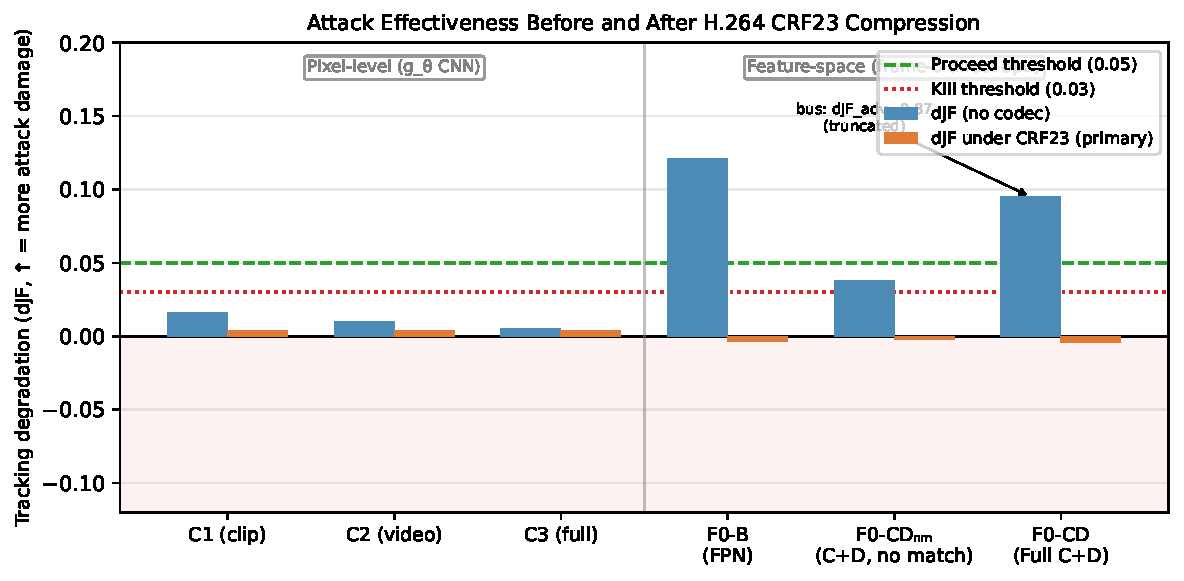
\includegraphics[width=\linewidth]{../figures/fig2_main_results.pdf}
\caption{Tracking degradation (dJF) before and after H.264 CRF23 compression across all six experiments. Blue bars: attack effectiveness without codec; orange bars: $\djfauc$ under CRF23 (primary metric). Dashed lines mark the proceed ($0.05$) and kill ($0.03$) thresholds. All orange bars fall below the kill threshold.}
\label{fig:main_results}
\end{figure}

\begin{figure}[t]
\centering
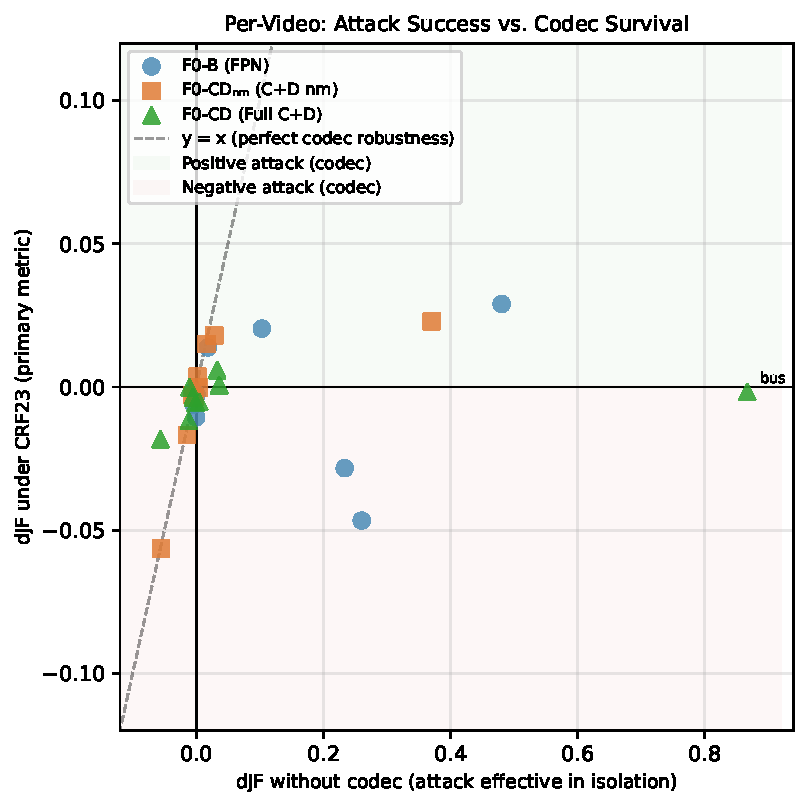
\includegraphics[width=0.9\linewidth]{../figures/fig4_scatter.pdf}
\caption{Per-video $\djfadv$ (x-axis) vs.\ $\djfauc$ (y-axis) for the three feature-space modes (27 data points). All attacks cluster near $y=0$ regardless of attack mode or per-video attack strength. The bus data point ($x=0.867$) illustrates that large optimizer-side attack strength does not predict codec survival.}
\label{fig:scatter}
\end{figure}
